% -----------------------------------------------------------------------------
\documentclass[a4paper]{artikel3}
% -----------------------------------------------------------------------------
\paperheight = 29.70 cm  \paperwidth = 21.0 cm  \hoffset        = 0.46 cm
\headheight  =  0.81 cm  \textwidth  = 15.0 cm  \evensidemargin = 0.00 cm
\headsep     =  0.81 cm	 \textheight = 9.00 in  \oddsidemargin  = 0.00 cm					
% -----------------------------------------------------------------------------
\usepackage[ruled,linesnumbered]{algorithm2e}
\usepackage{mathtools}
\usepackage{mathrsfs}
\usepackage{enumerate}
\usepackage{amsfonts}
\usepackage{amsmath}
\usepackage{amsthm}
\usepackage{amssymb}
\usepackage{url}
\usepackage{graphicx}
\usepackage{float}
\usepackage[font=small,labelfont=bf]{caption}
\usepackage{setspace}
\usepackage{booktabs}
\usepackage[pdfpagemode=None,
		    colorlinks=true, 
		    urlcolor=blue, 
		    linkcolor=blue, 
		    citecolor=blue, 
		    pdfstartview=FitH]{hyperref}
\usepackage{hyperref}
\hypersetup{
    colorlinks=true,
    linkcolor=blue,
    filecolor=magenta,      
    urlcolor=cyan,
    pdftitle={Overleaf Example},
    pdfpagemode=FullScreen,
    }
% -----------------------------------------------------------------------------
\newtheorem{theorem}{Theorem}
\newtheorem{corollary}[theorem]{Corollary}
\newtheorem{lemma}{Lemma}
\newtheorem{proposition}{Proposition}
\newtheorem{definition}[theorem]{Definition}
\newtheorem{remark}[theorem]{Remark}
\newtheorem{example}[theorem]{Example}
% -----------------------------------------------------------------------------
\newcommand{\norm}[1]{\left\Vert#1\right\Vert}
\newcommand{\abs}[1]{\left\vert#1\right\vert}
\newcommand{\set}[1]{\left\{#1\right\}}
\newcommand{\Real}{\mathbb R}
\newcommand{\Exp}{\mathbb E}
\newcommand{\eps}{\varepsilon}
\newcommand{\To}{\longrightarrow}
\newcommand{\mb}[1]{\mathbf{#1}}
\newcommand{\gb}[1]{\text{\boldmath$#1$}}
\newcommand{\ov}[1]{\overline{#1}}
\newcommand{\mml}{\{}
\newcommand{\mmr}{\}}
\newcommand{\lh}[1]{\widehat{#1}}
\newcommand{\pname}[1]{\textsc{#1}}
\newcommand{\lc}[1]{\mathscr{#1}}
\newcommand{\lcs}[1]{\ov{\mathscr{#1}}}
\newcommand{\lco}[1]{\overline{\mathscr{#1}}}
\newcommand{\lch}[1]{\widehat{\mathscr{#1}}}
\newcommand{\spi}{\ell}
\newcommand{\zf}[1]{z(#1)}

\newcommand{\R}{\mathbb{R}}    % Set of real numbers
\newcommand{\Z}{\mathbb{Z}}    % Set of integers
\renewcommand{\P}{\mathbb{P}}  % Probability measure
\newcommand{\I}{\mathbb{I}}    % Indicator function
\newcommand{\E}{\mathbb{E}}    % Expected value'

\newcommand{\F}{\mathscr{F}}   % Sigma-algebra
\renewcommand{\S}{\mathscr{S}} % Another sigma-algebra
\newcommand{\C}{\mathscr{C}}   % Collection of events

\numberwithin{equation}{section}
\numberwithin{theorem}{section}
\numberwithin{proposition}{section}
\numberwithin{lemma}{section}


% \newcommand{\if}{\text{if}}

% -----------------------------------------------------------------------------
\allowdisplaybreaks
\onehalfspacing
% -----------------------------------------------------------------------------

\begin{document}

{
\thispagestyle{empty}

{\large                       
Aalto University, Department of Finance
}

\vspace{5cm}               

{\huge \bf                    
Multidynamic model for yield curve estimation
}

\vspace{1cm}


{\large
Kasper Rantamäki
\par
kasper.rantamaki@aalto.fi}
}

\vspace{3.5cm}

{\large \bf
Abstract: \\
}
{
This study proposes a new parametric model for estimating yield curves. The model incorporates several key dynamics that influence the shape of the yield curve, including expectations of future yields, risk premia, and convexity. These dynamics are selected based on a literature review. The model is compared to two widely utilized yield curve models and is found to be more stable against outliers at the long- and short-ends of the yield curve. In addition, the information provided by the model in changing market environments is evaluated and found to be far more comprehensive than the contender models.
}


\vfill

{\large \today}


\clearpage


\thispagestyle{empty}


\tableofcontents


\clearpage


\section{Introduction}
\label{sec:intro}

\thispagestyle{empty}

Yield curves are a fundamental tool in fixed-income finance. They represent the yields of zero-coupon bonds across different maturities within a specified maturity range. In practice, however, yield curves are issuer-specific, meaning that only a limited number of bonds are available from which zero-coupon yields can be estimated. As a result, yields for intermediate maturities must be obtained through interpolation. This interpolation is non-trivial. Due to limits to arbitrage, observed zero-coupon yields may not align smoothly along a single curve. Consequently, a yield curve model must be fitted to the available observations to find a consistent and continuous yield curve. \\
\\
Two broad methodologies are commonly used to fit yield curves: spline-based methods and parametric models. The use of polynomial splines was pioneered by McCulloch \cite{mcculloch_1971}, with later developments by Waggoner \cite{waggoner_1997} and Anderson and Sleath \cite{anderson_sleath_1999}. Spline-based methods are highly flexible and can approximate almost any curve shape. However, this flexibility comes at a cost. Without appropriate smoothing or regularization, these models may overfit the observed data, producing yield curves that are economically unviable. \\
\\
Shea observed that McCulloch’s spline-based method tended to overfit at the ends of the maturity range \cite{shea_1984}. To address this issue, Nelson and Siegel proposed a parametric yield curve model \cite{nelson_siegel_1987}. They propose that under the expectations hypothesis, if spot rates are generated by a differential equation, the forward rates will be the solutions to the equation. They assume (without elaboration) that the instantenous forward rates solve a linear second order ordinary differential equation. Their model was later expanded by Svensson, who added a fourth term to the model \cite{svensson_1994}. \\
\\
The Nelson-Siegel model and, by association, the Svensson model suffer from their reliance on the expectation hypothesis. While Fama has found that the forward rates predict the future spot rate at a reasonable accuracy on the short-term (less than six months) \cite{fama_1984a}, this does not necessarily hold on the longer term. Indeed, Fama found that beyond 6-month maturity, a risk premium begins to influence the forward rates \cite{fama_1984b}. However, Fama also notes that the risk premium and expectations alone are insufficient to fully explain the observed shape of the yield curve. \\
\\
This study proposes an extension of the Nelson–Siegel model that incorporates additional dynamics affecting the shape of the yield curve. The selected dynamics are motivated by a brief literature review and are consistent with those proposed by Ilmanen and Iwanowski \cite{ilmanen_iwanowski_1997}. The inclusion of these additional components increases the model’s flexibility at the long-end of the maturity spectrum without a loss of granularity in the short-end. \\
\\
The proposed parametric model is compared with yield curve fitting methods commonly used in practice. Specifically, it is evaluated against the Anderson method \cite{anderson_sleath_1999}, which is implemented, for example, on the Refinitiv Workspace platform\footnote{To learn more, use the \texttt{<curvemethod>} command in the application}, and the Svensson model, which is used by several central banks \cite{bis_2005}. The comparison is based on statistical tests proposed by Anderson and Sleath \cite{anderson_sleath_1999}. The results indicate that the proposed model performs competitively relative to these contender models, while offering the additional advantage of more interpretable model parameters. \\
\\
This study is structured as follows. Chapter \ref{sec:hypotheses} contains a brief literature review of term-structure hypotheses, which are then applied when defining the proposed model. Chapter \ref{sec:contenders} introduces the contender models. The proposed model is defined in Chapter \ref{sec:model}. Chapter \ref{sec:tests} contains the statistical testing and comparison of the considered models. Finally, Chapter \ref{sec:conclusions} concludes the study. Additionally, Appendix \ref{app:bootstrap} outlines how the used yields were bootstrapped from observed bond prices. The regression method for finding the smoothing spline with varying penalty term used in the Anderson method is derived in Appendix \ref{app:varying_penalty_term}. The data used in the study is included in Appendix \ref{app:data}. The data was sourced from Refinitiv Workspace.

%Citations \cite{anderson_sleath_1999, christensen_sorensen_1994, cox_ingersoll_ross_1981, fama_1984a, fama_1984b, fama_bliss_1987, gurkaynak_et_al_2007, ilmanen_iwanowski_1997, mcculloch_1971, nelson_siegel_1987, shiller_1990, svensson_1994, waggoner_1997}


\clearpage


\section{Summary of term-structure hypotheses}
\label{sec:hypotheses}


The shape of the yield curve has been studied extensively (see, e.g., the examination by Cox, Ingersoll, and Ross \cite{cox_ingersoll_ross_1981}). This Chapter provides a brief high-level overview of these hypotheses. The hypotheses are often discussed in isolation, but in practice some combination of them (and potentially other hypotheses not listed here) determine the shape of the yield curve. For more discussion on combining these hypotheses, see, e.g, \cite{ilmanen_iwanowski_1997}.


\subsection{Pure expectations hypothesis}
\label{sec:expectations}


In its simplest form\footnote{There are many alternative forms of expectations hypothesis. For an overview, see, e.g., the literature review by Cox, Ingersoll and Ross \cite{cox_ingersoll_ross_1981}.}, the \emph{pure expectations hypothesis} is a no-arbitrage assumption that all bonds, independent of their time to maturity, earn the same near-term expected return. For example, assume there exists two zero-coupon bonds maturing at times $m_2$ and $m_1 < m_2$. The yields of these bonds are $y_1$ and $y_2$, respectively. If the bonds earn the same yield until maturity $m_1$, the forward rate between the maturities $m_1$ and $m_2$ must be $f_{m_1, m_2} = (y_2 m_2 - y_1 m_1) / (m_2 - m_2)$. This would be the yield that a zero-coupon bond with maturity in $m_2 - m_1$ years must earn $m_1$ years from now in order for the bond with maturity $m_2$ to break even. \\
\\
With the above reasoning, the yield curve at any arbitrary future point in time can be deduced from the current yield curve. However, this only holds if there is no stochasticity to the yields. In practice, the predictive power of forward rates is generally quite poor. Fama found that, while forward rates can predict the future spot rate quite well one month ahead, the quality of the predictions decreases after that and become unusable beyond five months \cite{fama_1984a}. This indicates that the expectations do contribute to the forward rates, but for longer maturities, they disappear among the other dynamics determining the yield curve shape.


\subsection{Liquidity preference hypothesis}
\label{sec:liquidity}


The \emph{liquidity preference hypothesis} was pioneered by Hicks \cite{hicks_1939}. He observed that borrowers prefer to issue long-term debt to ``hedge their future supplies of loan capital''. However, lenders (and institutions in that capacity) would prefer to lend short-term debt to ``keep their hands free to meet uncertainty''. Due to this discrepancy, the ``speculators'' that fill this offset demand a risk premium to do so. \\
\\
The risk premium is the spread between the expected return of the risky investment and its certainty equivalent. As a rational investor would always choose a portfolio with a greater return for a given level of risk, the risk premium should grow (monotonically) as a function of risk. With debt instruments, the risk to the lender grows with the time to maturity as the interest rates have more time to move, and there is more time for a sudden need for liquidity to arise for the lender. Thus, the expected return should grow as some (monotonic) function of time to maturity. \\
\\
Determining the shape of this risk-return function is non-trivial. Under the capital-asset pricing model (CAPM) \cite{sharpe_1964}, the expected return should grow linearly as a function of risk. The risk premium would then also grow linearly. If the markets were observed to behave as predicted by CAPM this would be a very clean theoretical result. However, this is generally not the case. \\
\\
Several studies have found that market frictions can cause non-monotonic behavior in the observed risk-return pairs, which goes against the predictions given by CAPM (see, e.g., \cite{baker_bradley_wurgler_2011, blitz_van_vliet_2007, frazzini_pedersen_2014}). Although these studies have focused on the equity markets, similar findings can be observed in the fixed-income markets as well. For example, Fama found that the expected return of U.S. Treasury Bills peaks at around 8 or 9 months, not at 12 months as a linear risk-return function would predict \cite{fama_1984b}. In isolation this seems to indicate that the risk premia is not a determining factor for the shape of the yield curve. However, as discussed by Ilmanen and Iwanowski \cite{ilmanen_iwanowski_1997}, the risk premium in conjunction with other dynamics can contribute to the shape of the yield curve. 


\subsection{Preferred habitat (market segmentation) hypothesis}
\label{sec:segmentation}


As discussed in Chapter \ref{sec:liquidity} the risk premia rarely behaves as predicted by standard financial theory. In equity markets, this is generally attributed to various market frictions \cite{baker_bradley_wurgler_2011, blitz_van_vliet_2007, frazzini_pedersen_2014}. However, with fixed income markets, an alternative explanation has also been proposed. \\
\\
In fixed income markets, market participants can have very different financing goals. In fact, this observations was the main motivation Hicks used when proposing the \emph{liquidity preference hypothesis} discussed in Chapter \ref{sec:liquidity}. Some of these market participants might invest in short-term debt, while others prefer long-term funding. Since these participants only inhabit a small maturity range, such ranges become effectively isolated. \\
\\
This idea was first put forward by Culbertson \cite{culbertson_1957} as \emph{market segmentation hypothesis}. Modigliani and Sutch \cite{modigliani_sutch_1966} built their \emph{preferred habitat theory} on the work by Culbertson, but with slightly relaxed assumptions. This study does not explore these hypotheses beyond their immediate implications to the risk premia. For more information, the reader is referred to the original articles or the literature review by Cox, Ingersoll and Ross \cite{cox_ingersoll_ross_1981}.\\
\\
If market participants are segmented, a single risk-return function will not explain the observed risk premiums. Instead, a preferred maturity weighted sum of investor specific risk premiums could potentially better match the observed marketwide risk premium. This would be some (potentially nonmonotonic) piecewise linear function. However, combining a large number of utility functions makes modeling significantly more challenging as the number of fittable parameters grows linearly. Some markets have an innate segmentation with bonds of various maturities that could be used as a proxy for such segmentation. A good example of this are the U.S. treasuries\footnote{Alternative example is the German government bonds, which are divided into Schatz, Bobl, and Bund. However, this division does not cover the whole maturity range and is thus not considered here further.}, which have the threefold division into T-Bills, T-Notes, and T-Bonds. For example, Waggoner \cite{waggoner_1997} defined the varying penalty term in his model based on these thresholds.


\subsection{Convexity bias}
\label{sec:convexity}


Yield curves can, at times, appear ``humped'', which means that the yield begins to decrease after some maturity. One explanation for this could be attributed to the market segmentation discussed in Chapter \ref{sec:segmentation}. Alternatively, the impact of convexity on the expected return of a bond can be used to explain the observed shape. \\
\\
Consider a second-order Taylor series expansion for a zero-coupon bond. The coefficient for the first order term is the duration and the coefficient for the second order term is (half of) convexity. For a zero-coupon bond, the convexity grows as the square of the time to maturity (assuming continuous compounding). Thus, it is always positive. Additionally, at the second order term the yield change is squared, meaning it is also always positive. Hence, the price impact of convexity is always positive regardless of the direction of the yield change. Investors should thus prefer a bond with higher convexity, \emph{ceteris paribus}.\\
\\
In line with the Taylor series expansion, the impact of convexity on the expected return is (half of) convexity times the square of the annualised volatility of the yield. Thus, an investor can accept a holding period return, and, by extension, yield, smaller by this amount while retaining the wanted expected return. Since the amount depends on the volatility, greater uncertainty in the future yield or, alternatively, an expected change in it, can decrease the current yield. This circles back to the pure expectations hypothesis discussed in Chapter \ref{sec:expectations} and shows that, especially as time to maturity grows, market expectations can disappear among other dynamics. 


\clearpage


\section{Contender models}
\label{sec:contenders}


\subsection{Svensson model}
\label{sec:svensson}


Svensson \cite{svensson_1994} proposed his model as a direct extension of the model by Nelson and Siegel \cite{nelson_siegel_1987}. The Nelson-Siegel model arises naturally from the few assumptions they impose. The fundamental assumption is that instantaneous forward rates are forecasts for future spot rates (in line with pure expectations hypophesis discussed Chapter \ref{sec:expectations}). Furthermore, they assume that the spot rates are generated by a second-order linear differential equation. Let $f_{NS}(m)$ be the instantaneous forward rate for maturity $m > 0$ under the Nelson-Siegel model. The differential equation is 

\begin{equation}
    \label{eq:nelson_siegel_eq}
    c_1 \frac{d^2 f_{NS}}{dt^2} + c_2\frac{df_{NS}}{dt} + c_3f_{NS} = c_4 ,
\end{equation}

where $c_i$ for $i \in \{1, 2, 3, 4\}$ are arbitrary coefficients. Assuming the differential equation in Equation \eqref{eq:nelson_siegel_eq} has a single real root, the forward rates have the general solution 

\begin{equation}
    \label{eq:nelson_siegel_sol}
    f_{NS}(m) = \beta_0 + \beta_1 \exp \left( -\frac{m}{\tau} \right) + \frac{\beta_2m}{\tau} \exp \left( -\frac{m}{\tau} \right) ,
\end{equation}

where $\tau$, $\beta_0$, $\beta_1$, and $\beta_2$ are coefficients associated with the solution. Nelson and Siegel observed that this single root solution provided a more parsimonious model and, thus, a better convergence when fitting for the coefficients than a solution with multiple roots. \\
\\
The zero-coupon yield under Nelson-Siegel model $r_{NS}(m)$ can be found as the average of the forward rates given by Equation \eqref{eq:nelson_siegel_sol}

\begin{equation*}
    r_{NS}(m) = \frac{1}{m}\int_0^m f_{NS}(s) ds .
\end{equation*}

Solving the above integral gives the final form for the Nelson-Siegel model

\begin{equation*}
    r_{NS}(m) = \beta_0 + \beta_1 \frac{1 - \exp \left( -m / \tau \right)}{m / \tau} + \beta_2 \left( \frac{1 - \exp \left( -m / \tau \right)}{m / \tau} - \exp \left( -\frac{m}{\tau} \right) \right) .
\end{equation*}

The Svensson model extends this by adding another second order term to the solution in Equation \eqref{eq:nelson_siegel_sol}. The zero-coupon yield under Svensson model $r_{S}(m)$ is outlined in Equation \eqref{eq:svensson_model}.

\begin{equation}
    \label{eq:svensson_model}
    \begin{aligned}
        r_{S}(m) &= \beta_0 + (\beta_1 + \beta_2) \frac{1 - \exp \left( -m / \tau_1 \right)}{m / \tau_1} - \beta_2 \left( \exp \left( -\frac{m}{\tau_1} \right) \right) \\
             &+ \beta_3 \left( \frac{1 - \exp \left( -m / \tau_2 \right)}{m / \tau_2} - \exp \left( -\frac{m}{\tau_2} \right) \right) . \\
    \end{aligned}
\end{equation}

The model coefficients can be found as the minimizers to a non-linear least squares problem. Since this is a common operation in statistics, it is not elaborated here. 


\clearpage


\subsection{Anderson method}
\label{sec:anderson}


Anderson and Sleath \cite{anderson_sleath_1999} propose using a a smoothing spline as an alternative to a parametric model. This idea had been explored before by, e.g., by Fisher, Nychka and Zervos \cite{fisher_nychka_zervos_1995} with the application of a regular (constant penalty) smoothing splines. The regular smoothing spline is found as the basis spline estimator $r_{FNZ}$ that minimizes the regularized weighted linear regression problem

\begin{equation}
    \label{eq:smoothing_spline}
    \sum_{i=1}^n w_i (y_i - r_{FNZ}(m_i))^2 + \lambda \int_{m_1}^{m_n} \left( \frac{d^2 r_{FNZ}}{d m^2}(u) \right)^2 du ,
\end{equation}

where $(m_i, y_i) \; \forall \; i \in \{1, 2,...,n\}$ are the data points (bootstrapped zero-coupon maturities and yields), $\mathbf{w}$ is a vector of weights and $\lambda$ is a regularization (penalty) parameter. To minimize the number of parameters to be estimated, unit weights are assumed, i.e., $\mathbf{w} = \mathbf{1}$. \\
\\
Similarly to the approach taken by Waggoner \cite{waggoner_1997}, the Anderson method uses a varying penalty (regularization) term. This changes the smoothing spline formulation in Equation \eqref{eq:smoothing_spline} to form 

\begin{equation}
    \label{eq:varying_penalty_term}
    \sum_{i=1}^n w_i (y_i - r_{A}(m_i))^2 + \int_{m_1}^{m_n} \lambda(u) \left( \frac{d^2 r_{A}}{d m^2}(u) \right)^2 du ,
\end{equation}

for some continuous function $\lambda(\cdot)$. Anderson and Sleath define the varying penalty term as 

\begin{equation*}
    \log(\lambda(m)) = a - (a - b)\exp(-m / c) ,
\end{equation*}

where $a$, $b$ and $c$ are parameters to be estimated. \\
\\
Note that the formulation in Equation \eqref{eq:varying_penalty_term} deviates slightly from that used by Anderson and Sleath. Anderson and Sleath chose to minimize the sum of squared yield residuals as 

\begin{equation*}
    X_P = \sum_{i=1}^N \left( \frac{P_i - \Pi_i}{D_i} \right)^2 ,
\end{equation*}

where $P_i$ is the observed price of bond $i$, $D_i$ its modified duration and $\Pi_i$ the fitted price. However, a more common choice, e.g., utilized in the Refinitiv implementation (see footnote in Chapter \ref{sec:intro}), is to fit the smoothing spline to bootstrapped zero-coupon yields. This approach will be taken in this study. The used bootstrapping algorithm is introduced in Appendix \ref{app:bootstrap}. \\
\\
Although the regular smoothing spline is quite commonly implemented in numerical analysis libraries (see, e.g., \texttt{scipy.interpolate.make\_smoothing\_spline} implementation \cite{scipy}), the varying penalty term is less common. The implementation used in this study is introduced in Appendix \ref{app:varying_penalty_term} and is based on the basis spline formulation introduced by de Boor \cite{de_boor_2003}.


\clearpage


\section{Proposed model}
\label{sec:model}


The proposed model takes inspiration from the Nelson-Siegel model, which was outlined in Chapter \ref{sec:svensson}. In fact, as the Nelson-Siegel model is defined purely based on the expectation hypothesis, it can be used to form the core of the model. However, the model additionally incorporates the risk (liquidity) premia and the convexity bias dynamics discussed in Chapters \ref{sec:liquidity} and \ref{sec:convexity}, respectively. \\
\\
The liquidity premia is some monotonically growing function of time to maturity. The exact shape of it depends on the level of risk aversion in the markets. However, under traditional financial theory (as discussed in Chapter \ref{sec:liquidity}), this shape can be assumed to be linear. Including this linear term in the forward rate function in Equation \eqref{eq:nelson_siegel_sol} yields

\begin{equation}
    \label{eq:proposed_forward_temp}
    f_{P}'(m) = \beta_0 + \beta_1 \exp \left( -\frac{m}{\tau} \right) + \frac{\beta_2m}{\tau} \exp \left( -\frac{m}{\tau} \right) + \beta_3' m .
\end{equation}

The convexity bias on the yield curve arises from the time value of convexity (see, e.g. \cite{christensen_sorensen_1994}). Convexity has a positive impact on the value of a bond when the yields change, \textit{ceteris paribus}. Hence, as convexity grows, an investor can accept a lower holding period return while maintaining the required level of expected returns. As discussed in Chapter \ref{sec:convexity} the convexity grows as the square of time to maturity for continuously compounded zero-coupon bonds. Incorporating this to the forward rate function in Equation \eqref{eq:proposed_forward_temp} gives

\begin{equation}
    \label{eq:proposed_forward}
    f_{P}(m) = \beta_0 + \beta_1 \exp \left( -\frac{m}{\tau} \right) + \frac{\beta_2m}{\tau} \exp \left( -\frac{m}{\tau} \right) + \beta_3' m - \beta_4' m^2 .
\end{equation}

The zero-coupon yield for this extension is

\begin{equation}
    \label{eq:proposed_model}
    r_{P}(m) =  \beta_0 + \frac{\tau}{m} (\beta_1 + \beta_2) \left(1 - \exp \left( - \frac{m}{\tau} \right) \right) - \beta_2 \exp \left( - \frac{m}{\tau} \right)  + \beta_3 m - \beta_4 m^2,
\end{equation}

where $\beta_3 = \frac{1}{2}\beta_3'$ and  $\beta_4 = \frac{1}{3}\beta_4'$. \\
\\
Consider the implication of the two additional terms for the model outlined in Equation \eqref{eq:proposed_model}. Without loss of generality, assume that $\beta_3 = \beta_4$. For maturities less than one year, the risk premia dominates and should be observable as a greater constituent for the expected return. However, for longer maturities, this effect is lost. Then, if an investor bases the expected returns purely on the yields, they should observe a peak at around one year to maturity. As discussed in Chapter \ref{sec:liquidity}, similar is observed in practice.


\clearpage


\section{Empirical testing}
\label{sec:tests}


Empirical testing of yield curve models is not possible in practice, since the ``correct'' yield curve is not known. Thus, testing must be done on surface level. The empirical evaluation of the model is done in two parts. Firstly, the model is compared to the contender models introduced in Chapter \ref{sec:contenders}. The comparison is done by evaluating how susceptible the models are to changes in the observed yields. Secondly, the information that can be inferred from the parameters of the proposed model is evaluated under different macroenvironments. \\
\\
The empirical evaluation is done using the closing quotes for the bonds and notes issued by the Republic of Finland. The Republic of Finland was chosen as the issuer, since the number of issued bonds is quite low, while still covering the full maturity range up to 30 years. The closing quotes and the bootstrapped zero-coupon yields for the date 2026-02-27 are included in the Appendix \ref{app:data} in Tables \ref{tab:bonds_20260227} and \ref{tab:yields_20260227}, respectively. These values are used in the analysis in Chapter \ref{sec:comparison}. The closing quotes and bootstrapped yields for the date 2026-03-06 are included in Tables \ref{tab:bonds_20260306} and \ref{tab:yields_20260306}, respectively. These are used as a point of comparison for the values from date 2026-02-27 in Chapter \ref{sec:information}. The dates were chosen to represent two different macroeconomic environments as on 2026-02-28, United States and Israel initiated the bombing of Iran, which led to an increase in general market uncertainty. The effect of this was observable both in the equity and fixed-income markets in Europe and the United States.


\subsection{Comparison to contender models}
\label{sec:comparison}


Anderson and Sleath \cite{anderson_sleath_1999} observe two deficiencies with the Svensson model, both of which are attributable to the flatness constraint at longer maturities. Firstly, in some cases, changing a single observation at the long-end of the maturity range has a significant impact on the model at the short-end. Secondly, the fit at the long-end can generally be quite poor. Both of these shortcomings are visible in Figure \ref{fig:shifted_long_end}. The graph on top shows the models fitted to the bootstrapped yields. Some observations can be made from it. Clearly, all of the models predict very similar yields for maturities ranging from around 5 to 15 years. However, deviations arise in the short and long ends. \\
\\
In the short-end, the Anderson method seems to provide the poorest fit. This results from the choice of knot points. How the points are chosen is non-trivial and can have a significant impact on the shape of the final curve. Anderson and Sleath use the maturities of every third bond as a knot point, following the approach set by Fischer, Nychka, and Zervos \cite{fisher_nychka_zervos_1995}. This study slightly deviates from that approach and uses uniformly distributed knot points. The number of knots is chosen to be half the number of bonds. The uniformly distributed knots were observed to be more computationally stable, but at the cost of granularity in the short-end. However, this does point to a general issue with spline based methods as they are, in the end, quite arbitrary. This makes them susceptible to poor convergence or poor fit, unless some specific decision are made when fitting for the data. However, justifying such decisions can be challenging. \\
\\
The Svensson model and the proposed model are almost identical in the short-end, but deviate slightly in the long-end. Between maturities of (roughly) 15 and 25 years, the proposed model slightly ``bulges'' out from the contender models. The cause for this appears to be the relatively high observed yield at the longest maturity, which otherwise would be far from the predicted yield. The yield predicted by the Svensson model also remains lower than the observed one, although not to the same extent. This is because the parametric form of the Svensson model can not provide upwards curvature at the long end. The only model that fits the last point reasonably well is the smoothing spline by Anderson and Sleath. While the varying penalty term penalises the curvature at the long end, there is no limitation for the shape that the spline can take there, which materializes as a better fit. \\
\\
The model fits change quite drastically when the last point is shifted down by (arbitrary) 30 bps as seen in the bottom graph of Figure \ref{fig:shifted_long_end}. The convexity term in the proposed model is able to fit the downwards trending long-end well, without causing issues in the short- and medium-term yields. The Svensson model is not as adabtable, which is observed as a deviation from the proposed model in the short-end (less than 2 years) and in the medium-term yields (between 5 and 15 years). The observed changes in the short-end are in line with the observations Anderson and Sleath made regarding the Svensson model \cite{anderson_sleath_1999}. The medium-term deviation in turn is similar to the bulging observed with the proposed model when fitted to the original data and is caused by the need for greater curvature at the long end. However, similarly to the Anderson method, the Svensson model still fails to fit the new shifted last point as well as the proposed model. \\
\\
These observations raise a concern regarding the \emph{goodness of fit} and the \emph{stability} of the models. Anderson and Sleath addressed these concerns with statistical testing. Anderson and Sleath propose using a leave one out cross-validation to measure the goodness of fit. This is discussed in more detail in Chapter \ref{sec:goodness_of_fit}. To measure the stability of the models, Anderson and Sleath suggest calculating the condition number for them. This methodology is discussed in Chapter \ref{sec:stability}.


\begin{figure}
    \centering
    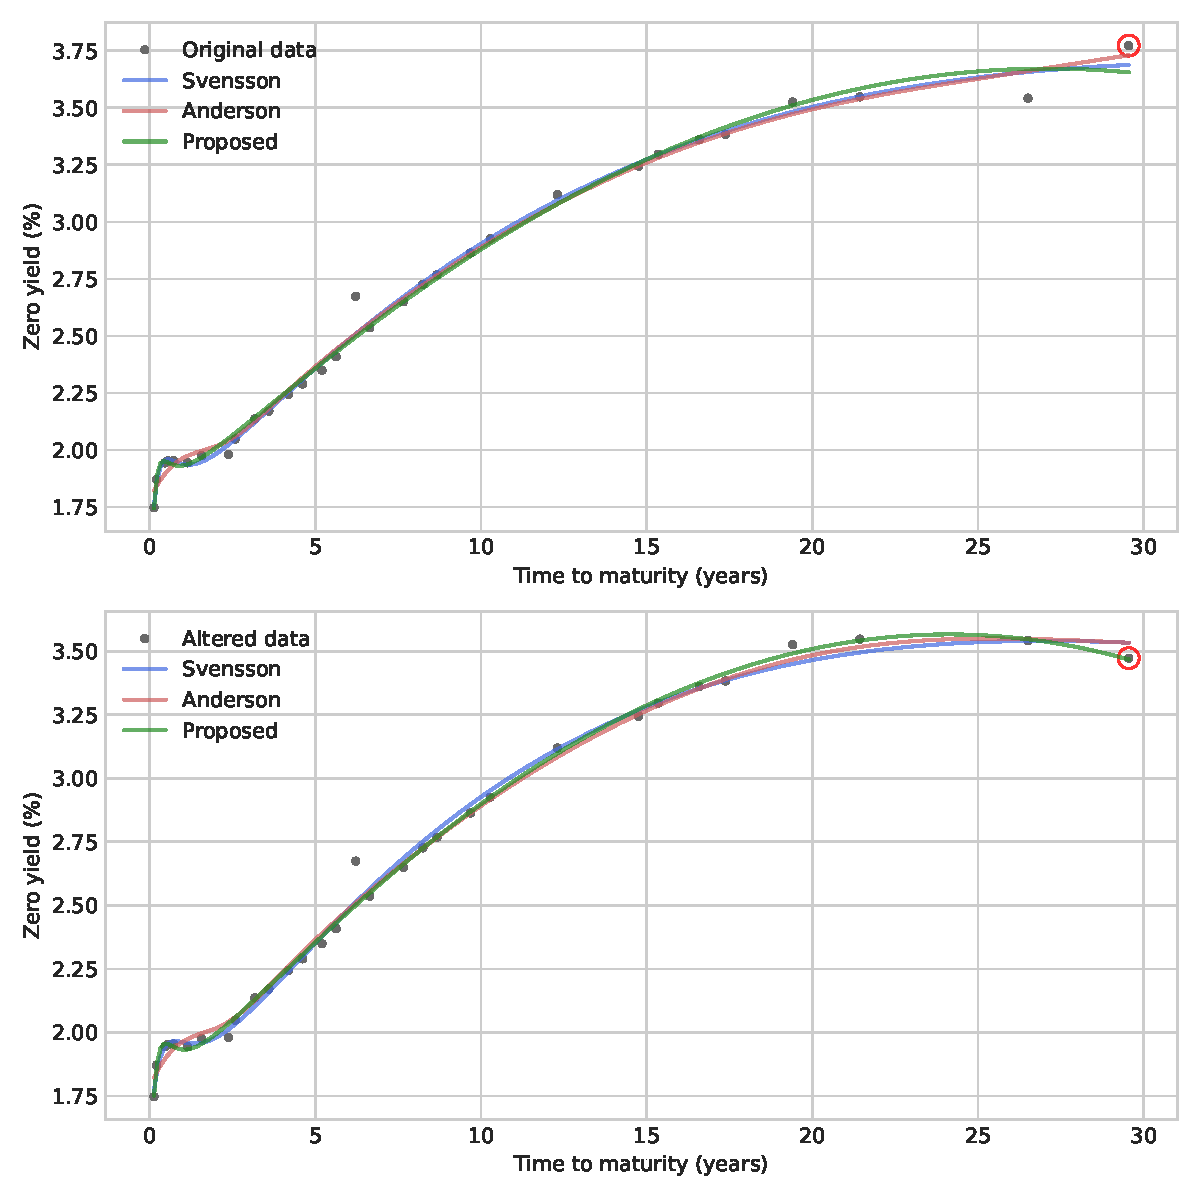
\includegraphics[scale=0.75]{Figures/01_shifted_long_end.pdf}
    \caption{The proposed model and the contender models fitted to the observed yields (top) and to the observed yields with 30 bps shift down at the longest maturity (bottom).}
    \label{fig:shifted_long_end}
\end{figure}


\subsubsection{Goodness of fit}
\label{sec:goodness_of_fit}


Anderson and Sleath propose using leave one out cross-validation to evaluate the goodness of fit for the models \cite{anderson_sleath_1999}. In leave one out cross-validation, as the name suggests, one observation is left out of the ``training set'' and is used to ``validate'' the trained model. In order to maintain the full maturity range, the longest and shortest maturity bonds are always kept in the ``training set''. The rest of the points are left out one at a time, and the absolute difference between the price of a 1EUR notional zero-coupon bond priced with the observed and predicted yield is calculated. The means and standard deviations for the absolute differences for each of the models are in Table \ref{tab:cv_all_bonds}.

\begin{table}[h!]
    \centering
    \begin{tabular}{| c | c | c |} 
    \hline
             & Mean              & Standard Deviation          \\
    \hline
    \hline
    Svensson & $0.00172$          & $0.00340$            \\
    \hline
    Anderson & $0.00200$          & $0.00370$            \\
    \hline
    Proposed & $0.00201$          & $0.00368$           \\
    \hline
    \end{tabular}
    \caption{The means and standard deviations the absolute differences in prices of 1EUR notional zero-coupon bonds when priced with the observed yield and the predicted yield found in a leave one out cross validation.}
    \label{tab:cv_all_bonds}
\end{table}

The means and standard deviations are very similar for all models, with the Svensson model having slightly better goodness of fit. However, independent of the model, the fit is very good, leading to an average difference in the bond prices of around $0.2$ cents. Still, even this is mainly attributable to the hard to fit longest maturity bond. The means and standard deviations for the leave one out cross-validation, when the longest maturity observation is excluded, are in Table \ref{tab:cv_exc_bonds}.

\begin{table}[h!]
    \centering
    \begin{tabular}{| c | c | c |} 
    \hline
             & Mean              & Standard Deviation          \\
    \hline
    \hline
    Svensson & $0.00151$          & $0.00209$            \\
    \hline
    Anderson & $0.00136$          & $0.00203$            \\
    \hline
    Proposed & $0.00127$          & $0.00195$           \\
    \hline
    \end{tabular}
    \caption{The means and standard deviations the absolute differences in prices of 1EUR notional zero-coupon bonds when priced with the observed yield and the predicted yield found in a leave one out cross validation. The longest maturity point was excluded from the observation set.}
    \label{tab:cv_exc_bonds}
\end{table}

When excluding the longest maturity bond, the proposed model provides the best fit, while the Svensson model performs worst. However, all models improve when compared to the test with all bonds. The found average difference in bond prices is only around $0.15$ cents, with smaller deviations. This indicates that the fit that can be achieved with the proposed model is comparable and competitive with the contender models. 


\subsubsection{Stability}
\label{sec:stability}

Anderson and Sleath propose measuring the stability of a model with its condition number \cite{anderson_sleath_1999}. The condition number quantifies the ratio between how much the output of a function changes for a given change in the input. Let $g : \R \mapsto \R$ be some function of a single variable $x$. Anderson and Sleath use the relative condition number $\kappa$, which for the function $g$ is given by 

\begin{equation*}
    \kappa_g(x) = \frac{x}{\Delta x}\frac{g(x + \Delta x) - g(x)}{g(x)} ,
\end{equation*}

where $\Delta x$ is the change in the input. \\
\\
Anderson and Sleath compute the average and maximum yields for the curves found with the original and the perturbated bond prices and use these to find the condition number. This seems unnecessary, and instead the condition number is calculated as the Euclidean norm of the condition numbers evaluated at the bond maturities. More formally, for a given yield curve model $r$ and bonds with maturities $\mathbf{m}$ the condition number is given by

\begin{equation*}
    \kappa_r = \left\| \frac{\mathbf{y}}{\mathbf{e}} \frac{r^{(\mathbf{e})}(\mathbf{m}) - r(\mathbf{m})}{r(\mathbf{m})} \right\|_2 ,
\end{equation*}

where the division, multiplication and subtraction are done elementwise and $r^{(\mathbf{e})}$ is the yield curve found with noise vector $\mathbf{e}$ added to the input yields $\mathbf{y}$. \\
\\
The condition numbers are computed for each of the considered models, with i.i.d. normally distributed noise $e \sim \mathcal{N}(0, SD(\mathbf{y}) / 10)$ added to the input yields. This simulation is done 100 times and the mean condition number for each model is calculated. These mean condition numbers are listed in Table \ref{tab:condition_numbers}.

\begin{table}[h!]
    \centering
    \begin{tabular}{| c | c |} 
    \hline
    Model    & Condition number  \\
    \hline
    \hline
    Svensson & $16.514$         \\
    \hline
    Anderson & $14.498$         \\
    \hline
    Proposed & $15.594$         \\
    \hline
    \end{tabular}
    \caption{The found condition numbers for the considered models.}
    \label{tab:condition_numbers}
\end{table}


The condition numbers are of similar magnitude to what Anderson and Sleath found for their considered models. The condition number for the proposed model is almost exactly half way between the condition numbers of the contender models. This makes it a competitive, but not a particularly stable model. Generally, Anderson and Sleath found that parsimonius models, like the Nelson-Siegel model or the smoothing spline proposed by Fischer, Nychka and Zervos are more stable, but this stability comes at the cost of granularity, i.e., with worse goodness of fit. 


\subsection{Information on the yield curve}
\label{sec:information}


In contrast to the contender models, the terms in the proposed model represent different dynamics that govern the shape of the yield curve. Thus, when the yield curve evolves with time, the drivers for the change can be isolated. As an example of this, the yields bootstrapped from the prices of the bonds and notes issued by the Republic of Finland on 2026-02-27 and 2026-03-06 are considered. These yields and the fitted proposed model are in Figure \ref{fig:date_comp}. The parameters of the fitted models are in Table \ref{tab:date_comp_params}. 


\begin{figure}
    \centering
    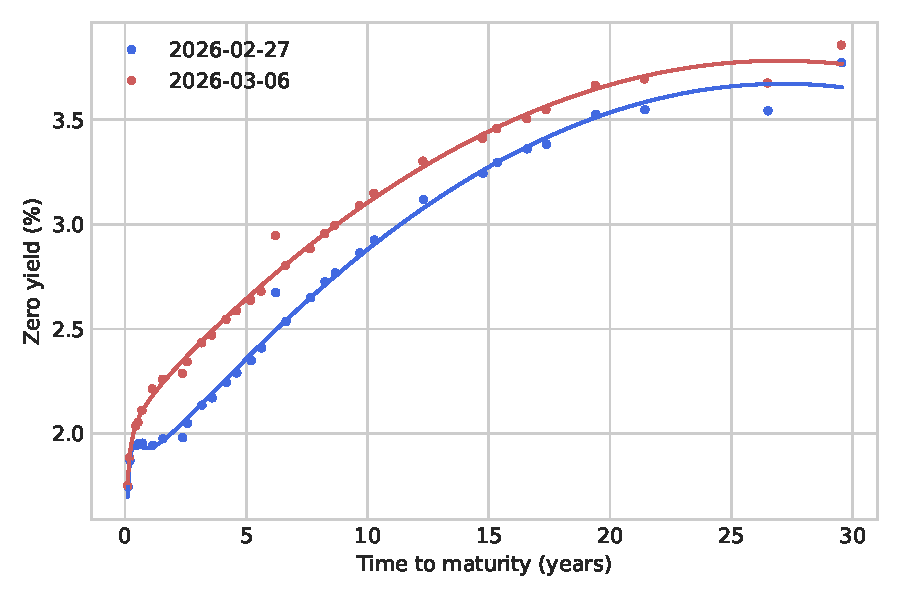
\includegraphics[scale=0.8]{Figures/02_date_comp.pdf}
    \caption{The bootstrapped yields from Tables \ref{tab:yields_20260227} and \ref{tab:yields_20260306} and the fitted proposed models.}
    \label{fig:date_comp}
\end{figure}


\begin{table}[h!]
    \centering
    \begin{tabular}{| c | c | c |} 
    \hline
    Parameter & 2026-02-27        & 2026-03-06          \\
    \hline
    \hline
    $\tau$    & $0.1315$          & $0.0561$            \\
    \hline
    $\beta_0$ & $0.0166$          & $0.0208$            \\
    \hline
    $\beta_1$ & $-0.0051$         & $-0.0076$           \\
    \hline
    $\beta_2$ & $0.0148$          & $2.6\cdot10^{-6}$   \\
    \hline
    $\beta_3$ & $0.0015$          & $0.0013$            \\
    \hline
    $\beta_4$ & $2.7\cdot10^{-5}$ & $2.3\cdot10^{-5}$   \\
    \hline
    \end{tabular}
    \caption{The parameter values for the fitted models seen in Figure \ref{fig:date_comp}.}
    \label{tab:date_comp_params}
\end{table}


The model parameters are clearly different between the dates. However, to better understand what these parameters tell about the yield curve, following the example set by Nelson and Siegel \cite{nelson_siegel_1987}, the \emph{forward} curve is decomposed to its constituent parts. These decompositions are in Figure \ref{fig:forward_breakdown}.


\begin{figure}
    \centering
    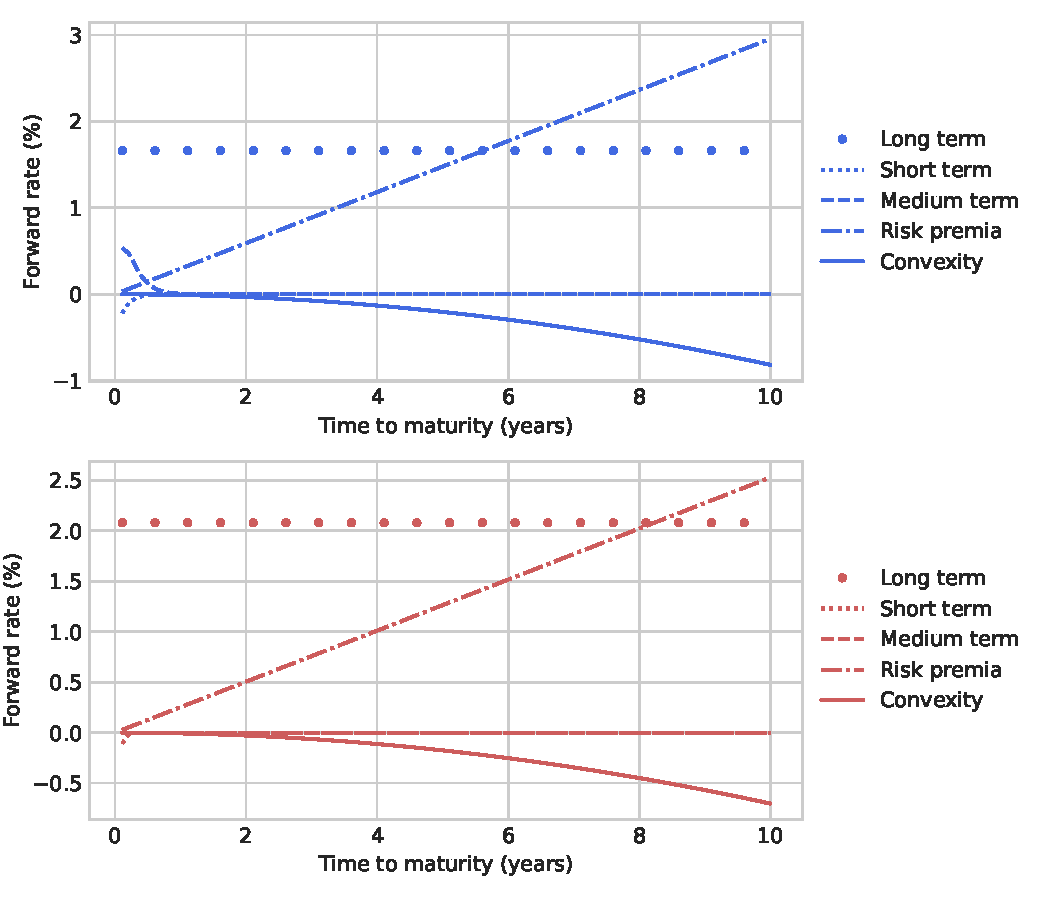
\includegraphics[scale=0.8]{Figures/02_forward_breakdown.pdf}
    \caption{The decomposed forward curves for the dates 2026-02-27 (top) and 2026-03-06 (bottom).}
    \label{fig:forward_breakdown}
\end{figure}


Consider the forward curve expression in Equation \eqref{eq:proposed_forward}. The long-term interest rate level is governed by the parameter $\beta_0$. This term increased by around $40$ bps from 2026-02-27 to 2026-03-06, which signifies an increased yield requirement across the curve. This increase is most likely caused by general flight-to-liquidity or flight-to-quality phenomenon seen during periods of increased market uncertainty. \\
\\
The short-term dynamic is given by the term $\beta_1 \exp \left( -\frac{m}{\tau} \right)$ in Equation \eqref{eq:proposed_forward}. The deacrease of both $\tau$ and $\beta_1$ make it far less prominent on 2026-03-06 when compared to 2026-02-27. Same can be seen to an even greater extent in the medium-term dynamic given by the term $\frac{\beta_2m}{\tau} \exp \left( -\frac{m}{\tau} \right)$ as the parameter $\beta_2$ becomes almost zero on 2026-03-06. These two terms come from the Nelson-Siegel model on which the proposed model is built. Thus, they represent the pure expectations hypothesis in the model. The decrease in the $\beta_1$ and $\beta_2$ parameters signals that the expectations hypothesis gets obfuscated by the other dynamics, which, under market uncertainty, is to be expected. \\
\\
Finally, the parameters $\beta_3$ and $\beta_4$ govern the risk premia and the convexity dynamics, respectively. These parameters remain relatively constant from 2026-02-27 until 2026-03-06, which means that the general increase in market uncertainty is mainly incapsulated in the increased long term interest rate level. This is a reasonable result as, for example, under capital asset pricing model the slope of the capital market line should be mostly constant, and a general increase in the risk level should push all assets up the capital market line, without changing its slope. Similar, holds for the convexity term. Thus, the forward curves tell that, even without knowing anything about the macroenvironment, the market uncertainty increased significantly, which decreased the predictive power of the short-term expected values.



\clearpage


\section{Conclusions}
\label{sec:conclusions}


This study proposes a new parametric model for yield curve estimation. The key insight behind the model definition is the set of term-structure hypotheses which together can explain the observed shape of the yield curve. Incorporating these insights results in a model that is more stable than the Svensson model while achieving a similar or improved goodness of fit. The proposed model is able to achieve this while retaining the same number of estimated parameters. \\
\\
The main advantage of the proposed model is its interpretability. In spline-based models, the coefficients of the basis splines do not convey information about the underlying causes for the shape the curve, making the curve largely arbitrary. Similarly, some parametric models, such as the Svensson model, introduce additional terms without clear theoretical justification, which can obscure the information the curve can provide. In contrast, the proposed model avoids these issues, as its components are directly motivated by established term-structure dynamics. \\
\\
For the bonds examined in this study, the proposed model achieves goodness of fit and stability comparable to smoothing spline methods, while retaining the simplicity of a parametric model. This makes it a competitive option for institutions that require consistent and reliable yield curve estimates. Additionally, the constraints implied by the incorporated dynamics ensure that the resulting yield curves remain ``realistic'' under the assumed term-structure hypotheses. Spline-based methods lack such constraints and may therefore produce undesirable features, such as oscillatory or “wavy” curves. Avoiding these artifacts often requires adjusting knot placements or modifying penalty parameters. Such fine-tuning introduces a degree of subjectivity, as practitioners must judge what constitutes a reasonable curve shape. By contrast, the proposed model provides a theory-driven approach to yield curve estimation while maintaining practical flexibility.


\clearpage


\bibliographystyle{ieeetr}
\bibliography{library}


\clearpage


\appendix


\section{Bootstrapping}
\label{app:bootstrap}


Bootstrapping can be approached either via iterative forward substitution or a system of linear equations. This appendix introduces the linear system approach. Assume that there exist $N$ fixed-coupon bonds from the same issuer. Without loss of generality, assume that each bond pays an annual coupon. In addition, assume that the bonds mature on the same day of the year. Thus, the coupon payments occur on days in set $T = \{t_1, t_2, ..., t_N \}$. This might seem like a restrictive assumption, but is commonly observed in practice (see, e.g., Table \ref{tab:bonds_20260227}). \\
\\
Denote the price of a bond maturing at time $t_i \in T$ by $P_i$. By the assumptions established above, the bond $i$ provides cashflows at all times $t_j \leq t_i$ where $t_j \in T$. Represent these cashflows by a vector $\mathbf{c}_i$, such that the cashflow $c_{i,j}$ is paid at time $t_j \in T$. If the price of a zero-coupon bond is modeled purely by discounting, then the price of bond $i$ can be written as

\begin{equation*}
    P_i = 
    \begin{bmatrix}
        \mathbf{c}_{i} \\
        \mathbf{0}_{N-i}
    \end{bmatrix}^\top \mathbf{d} ,
\end{equation*}

where $\top$ denotes matrix transpose, $\mathbf{d} \in [0, 1]^N$ is a vector of discount factors and $\mathbf{0}_{N-i}$ is an appropriately sized vector of zeros to extend the dimension of vector $\mathbf{c}_{i}$ to $N$. \\
\\
Since the prices of the bonds are known, the discount factors can be solved from the linear system

\begin{equation}
    \label{eq:basic_bootstrap}
    \mathbf{P} = 
    \begin{bmatrix}
        \mathbf{c}_{1}^\top & \mathbf{0}_{N-1}^\top \\
        \mathbf{c}_{2}^\top & \mathbf{0}_{N-2}^\top \\
        \vdots           & \vdots             \\
        \mathbf{c}_{N}^\top & \mathbf{0}_{0}^\top   \\
    \end{bmatrix} \mathbf{d} ,
\end{equation}

where $\mathbf{P} \in \R^N$ is a vector containing the observed bond prices. \\
\\
The system in Equation \eqref{eq:basic_bootstrap} provides a unique solution for the discount factors iff there exists a maturing bond for each coupon date. Often a subset of the issued bonds that satisfy this condition can be found up to some maturity. However, this might not be enough to form the full yield curve for maturities of 20, 30, or even 40 to 50 years. In such cases, the discount factor has to be interpolated from the points around it. This is illustrated in the following example with the use of linear interpolation. \\
\\
Consider two bonds with observed prices $P_1$ and $P_3$ and cashflow vectors $\mathbf{c}_1 = [c_{1, 1}]$ and $\mathbf{c}_3 = [c_{3, 1} \quad c_{3, 2} \quad c_{3, 3}]^\top$. Clearly, the discount factors can not be found with the linear system in Equation \eqref{eq:basic_bootstrap}, as there are two observations, but three unknowns. This becomes clearer when the system is written open

\begin{equation*}
    \begin{bmatrix}
        P_1 \\
        P_3 \\
    \end{bmatrix} = 
    \begin{bmatrix}
        c_{1, 1} & 0        & 0        \\
        c_{3, 1} & c_{3, 2} & c_{3, 3} \\
    \end{bmatrix} 
    \begin{bmatrix}
        d_1 \\
        d_2 \\
        d_3 \\
    \end{bmatrix} = 
    \begin{bmatrix}
        c_{1, 1}d_1 + 0 + 0 \\
        c_{3, 1}d_1 + c_{3, 2}d_2 + c_{3, 3}d_3 \\
    \end{bmatrix} .
\end{equation*}

The system becomes solvable if the discount factor $d_2$ is assumed to be representable as some combination of the discount factors $d_1$ and $d_3$. If this combination is assumed to be linear (i.e., linear interpolation is applied), the discount factor $d_2$ can be replaced with $(d_1 + d_3)/2$. This results in a (solvable) linear system

\begin{equation*}
    \begin{bmatrix}
        P_1 \\
        P_3 \\
    \end{bmatrix} = 
    \begin{bmatrix}
        c_{1, 1}d_1 \\
        d_1\left( c_{3, 1} + \frac{c_{3, 2}}{2} \right) + d_3\left( c_{3, 3} + \frac{c_{3, 2}}{2} \right) \\
    \end{bmatrix} =
    \begin{bmatrix}
        c_{1, 1}                      & 0                             \\
        c_{3, 1} + \frac{c_{3, 2}}{2} & c_{3, 3} + \frac{c_{3, 2}}{2} \\
    \end{bmatrix} 
    \begin{bmatrix}
        d_1 \\
        d_3 \\
    \end{bmatrix}
     .
\end{equation*}

Extending this methodology to an arbitrary number of bonds is trivial.


\clearpage


\section{Smoothing splines with varying penalty term}
\label{app:varying_penalty_term}


The varying penalty term is presented as a generalization of the regular smoothing spline problem formulated in Equation \eqref{eq:smoothing_spline}. This in turn is defined using basis splines. Suppose there exists noisy observations $\mathbf{y} \in \R^n$ of some phenomena with a single explanatory variable $x$ with observed values $\mathbf{x} \in \R^n$. The goal is to find a smooth estimator $\hat{f}$ for the unknown function $f$ which generated the data. \\
\\
Smoothing splines are represented as a series of basis splines (B-splines). Each B-spline $i$ of order $p +1$ is a collection of piecewise polynomial functions of order-$p$. The values $\mathbf{t} = [t_0 \quad t_1 \quad ... \quad t_k]$, where these piecewise polynomials meet, are called knots. A given B-spline $B_i^{(p)}(x)$ of order $p$ is non-zero within the range $[t_i, t_{i+p+1}]$. De Boor \cite{de_boor_2003} proposes defining such B-splines recursively with the base condition 

\begin{equation*}
    B_i^{(0)}(x) = 
    \begin{cases}
        1 & \text{if } t_i \leq x < t_{i+1} \\
        0 & \text{otherwise},
    \end{cases}
\end{equation*}

and recursion step

\begin{equation*}
    B_i^{(p)}(x) = \frac{x - t_i}{t_{i + p} - t_{i}}B_i^{(p-1)}(x) + \frac{t_{i + p + 1} - x}{t_{i + p + 1} - t_{i + 1}}B_{i + 1}^{(p-1)}(x) .
\end{equation*}

Any given spline function can be represented as a sum of basis splines. Let the number of basis splines of order-$p$  be $N$. The estimator spline is then

\begin{equation*}
    \hat{f}(\mathbf{x)} = \sum_{i=1}^N a_i B_i^{(p)}(\mathbf{x)} .
\end{equation*}

This estimator can be used to form a linear system 

\begin{equation*}
    \mathbf{y} = \mathbf{B} \mathbf{a} + \epsilon ,
\end{equation*}

where matrix $\mathbf{B} \in \R^{n \times N}$ contains the B-spline values, i.e., $B_{ij} = B_j^{(p)}(x_i)$. The least squares minimizer for the coefficients $\mathbf{a}$ can be found by solving the system of normal equations

\begin{equation*}
    \mathbf{B}^\top \mathbf{B} \mathbf{a} = \mathbf{B}^\top \mathbf{y} .
\end{equation*}

This solution corresponds with solving the regression problem in Equation \eqref{eq:smoothing_spline}, when the weights $\mathbf{w}$ are all ones and the penalty term is $\lambda = 0$. An additional term needs to be added when the penalty term is non-zero. The second derivative of the estimator spline is 

\begin{equation*}
    \hat{f}''(\mathbf{x}) = \sum_{i=1}^N a_i \frac{d^2 B_i^{(p)}}{d x^2}(\mathbf{x)} .
\end{equation*}

Assume that the order of the B-splines is $p=3$ (cubic splines). The integral term can be written as

\begin{equation}
    \label{eq:regular_penalty_term}
    \lambda\int_{x_1}^{x_n} \left( \hat{f}''(s) \right)^2 \; ds = \lambda \sum_{i=1}^N a_i \left[ \sum_{j=1}^N a_j \int_{x_1}^{x_n} \frac{d^2 B_i^{(3)}}{d x^2}(s) \frac{d^2 B_j^{(3)}}{d x^2}(s) \; ds \right] .
\end{equation}

Consider a matrix $\mathbf{L} \in \R^{N \times N}$ with elements 

\begin{equation}
    \label{eq:matrix_elems}
    L_{i, j} = \int_{x_1}^{x_n} \frac{d^2 B_i^{(3)}}{d x^2}(s) \frac{d^2 B_j^{(3)}}{d x^2}(s) \; ds .
\end{equation}

Then the expression from Equation \eqref{eq:regular_penalty_term} can be written in form

\begin{equation*}
    \lambda \sum_{i=1}^N a_i \left[ \sum_{j=1}^N a_j \int_{x_1}^{x_n} \frac{d^2 B_i^{(3)}}{d x^2}(s) \frac{d^2 B_j^{(3)}}{d x^2}(s) \; ds \right] = \lambda \mathbf{a}^\top \mathbf{L} \mathbf{a} .
\end{equation*}

Generalization from a constant penalty term to a varying one can be achieved by modifying the definition of the matrix elements in Equation \eqref{eq:matrix_elems}. This leads to a new matrix with elements 

\begin{equation*}
    L'_{i, j} = \int_{x_1}^{x_n} \lambda(s) \frac{d^2 B_i^{(3)}}{d x^2}(s) \frac{d^2 B_j^{(3)}}{d x^2}(s) \; ds .
\end{equation*}

The elements in the matrix $\mathbf{L}'$ can be solved with numerical integration methods. The final problem formulation is

\begin{equation}
    \label{eq:smoothing_spline_regression}
    \sum_{i=1}^n w_i (y_i - \hat{f}(m_i))^2 + \int_{x_1}^{x_n} \lambda(s) (\hat{f}''(s))^2 \; ds = (\mathbf{y} - \mathbf{B} \mathbf{a})^\top \mathbf{W} (\mathbf{y} - \mathbf{B} \mathbf{a}) + \mathbf{a}^\top \mathbf{L}' \mathbf{a} ,
\end{equation}

where $\mathbf{W} = \text{diag}(\mathbf{w})$ is a matrix with the weights $\mathbf{w}$ on its diagonal. To solve the problem in Equation \eqref{eq:smoothing_spline_regression} define a loss term $l$ as 

\begin{equation*}
    \begin{aligned}
        l &= (\mathbf{y} - \mathbf{B} \mathbf{a})^\top \mathbf{W} (\mathbf{y} - \mathbf{B} \mathbf{a}) + \mathbf{a}^\top \mathbf{L}' \mathbf{a} \\
          &= \mathbf{y}^\top \mathbf{W} \mathbf{y} - 2\mathbf{a}^\top \mathbf{B}^\top \mathbf{W} \mathbf{y} + \mathbf{a}^\top \mathbf{B}^\top \mathbf{W} \mathbf{B}\mathbf{a} + \mathbf{a}^\top \mathbf{L}' \mathbf{a} .
    \end{aligned}
\end{equation*}

The gradient of the loss is 

\begin{equation*}
    \frac{\partial l}{\partial \mathbf{a}} = 2(\mathbf{B}^\top \mathbf{W} \mathbf{B}\mathbf{a} + \mathbf{L}' \mathbf{a} - \mathbf{B}^\top \mathbf{W} \mathbf{y}) .
\end{equation*}

The problem is minimized when the gradient is zero. Coefficients for the minimizer are 

\begin{equation*}
    (\mathbf{B}^\top \mathbf{W} \mathbf{B} + \mathbf{L}') \mathbf{a} = \mathbf{B}^\top \mathbf{W} \mathbf{y} \implies \mathbf{a} = (\mathbf{B}^\top \mathbf{W} \mathbf{B} + \mathbf{L}')^{-1}\mathbf{B}^\top \mathbf{W} \mathbf{y} .
\end{equation*}


\clearpage


\section{Data}
\label{app:data}


\begin{table}[h!]
    \centering
    \begin{tabular}{| c | c | c | c | c | c | c |} 
\hline
ISIN & Coupon Rate (\%) & Maturity Date & Issue Date & Bid & Ask & Accrual \\
\hline
\hline
FI4000197959 & 0.5 & 2026-04-15 & 2016-03-08 & 99.76 & 99.9 & 0.4411 \\
\hline
FI4000590971 & 0.0 & 2026-05-13 & 2025-06-05 & 99.607 & 99.615 & 0.0 \\
\hline
FI4000592183 & 0.0 & 2026-08-13 & 2025-09-11 & 99.095 & 99.11 & 0.0 \\
\hline
FI4000511449 & 0.0 & 2026-09-15 & 2021-08-31 & 98.898 & 98.944 & 0.0 \\
\hline
FI4000598396 & 0.0 & 2026-11-13 & 2026-01-09 & 98.57 & 98.638 & 0.0 \\
\hline
FI4000527551 & 1.375 & 2027-04-15 & 2022-08-30 & 99.244 & 99.364 & 1.213 \\
\hline
FI4000278551 & 0.5 & 2027-09-15 & 2017-09-06 & 97.636 & 97.756 & 0.2315 \\
\hline
FI4000037635 & 2.75 & 2028-07-04 & 2012-02-07 & 101.542 & 101.662 & 1.8233 \\
\hline
FI4000348727 & 0.5 & 2028-09-15 & 2018-09-04 & 96.003 & 96.123 & 0.2315 \\
\hline
FI4000557525 & 2.875 & 2029-04-15 & 2023-08-30 & 101.989 & 102.109 & 2.5363 \\
\hline
FI4000369467 & 0.5 & 2029-09-15 & 2019-02-12 & 94.108 & 94.228 & 0.2315 \\
\hline
FI4000577952 & 2.5 & 2030-04-15 & 2024-08-27 & 100.775 & 100.785 & 2.2123 \\
\hline
FI4000441878 & 0.0 & 2030-09-15 & 2020-09-02 & 89.901 & 90.051 & 0.0 \\
\hline
FI4000148630 & 0.75 & 2031-04-15 & 2015-03-10 & 92.027 & 92.147 & 0.6616 \\
\hline
FI4000507231 & 0.125 & 2031-09-15 & 2021-05-26 & 87.892 & 88.042 & 0.0579 \\
\hline
FI4000591862 & 2.625 & 2032-04-15 & 2025-08-28 & 100.368 & 100.518 & 1.3449 \\
\hline
FI4000523238 & 1.5 & 2032-09-15 & 2022-06-01 & 93.371 & 93.571 & 0.6945 \\
\hline
FI4000550249 & 3.0 & 2033-09-15 & 2023-05-04 & 101.969 & 102.119 & 1.389 \\
\hline
FI4000306758 & 1.125 & 2034-04-15 & 2018-02-13 & 87.967 & 88.117 & 0.9925 \\
\hline
FI4000571104 & 3.0 & 2034-09-15 & 2024-04-30 & 101.355 & 101.505 & 1.389 \\
\hline
FI4000587415 & 3.0 & 2035-09-15 & 2025-05-07 & 100.747 & 100.897 & 1.389 \\
\hline
FI4000415153 & 0.125 & 2036-04-15 & 2020-02-11 & 75.071 & 75.191 & 0.1103 \\
\hline
FI4000546528 & 2.75 & 2038-04-15 & 2023-02-02 & 96.055 & 96.154 & 2.426 \\
\hline
FI4000440557 & 0.25 & 2040-09-15 & 2020-06-17 & 64.817 & 64.917 & 0.1158 \\
\hline
FI4000598776 & 3.55 & 2041-04-15 & 2026-01-28 & 102.436 & 102.536 & 0.3307 \\
\hline
FI4000046545 & 2.625 & 2042-07-04 & 2012-07-03 & 90.612 & 90.812 & 1.7404 \\
\hline
FI4000517677 & 0.5 & 2043-04-15 & 2022-02-02 & 62.077 & 62.277 & 0.4411 \\
\hline
FI4000586284 & 3.2 & 2045-04-15 & 2025-01-29 & 96.092 & 96.192 & 2.823 \\
\hline
FI4000242870 & 1.375 & 2047-04-15 & 2017-02-15 & 67.608 & 67.768 & 1.213 \\
\hline
FI4000480488 & 0.125 & 2052-04-15 & 2021-02-09 & 41.165 & 41.365 & 0.1103 \\
\hline
FI4000566294 & 2.95 & 2055-04-15 & 2024-01-24 & 86.919 & 87.159 & 2.6025 \\
\hline
    \end{tabular}
    \caption{The closing quotes for the bonds and notes issued by the The Republic of Finland, on 2026-02-27. The quotes were sourced from Refinitiv (LSEG Datastream). The bonds are EUR denominated and pay an annual coupon.}
    \label{tab:bonds_20260227}
\end{table}


\begin{table}[h!]
    \centering
    \begin{tabular}{| c | c | c | c | c | c | c |} 
\hline
ISIN & Coupon Rate (\%) & Maturity Date & Issue Date & Bid & Ask & Accrual  \\
\hline
\hline
FI4000197959 & 0.5 & 2026-04-15 & 2016-03-08 & 99.819 & 99.889 & 0.4507 \\
\hline
FI4000590971 & 0.0 & 2026-05-13 & 2025-06-05 & 99.641 & 99.648 & 0.0 \\
\hline
FI4000592183 & 0.0 & 2026-08-13 & 2025-09-11 & 99.078 & 99.12 & 0.0 \\
\hline
FI4000511449 & 0.0 & 2026-09-15 & 2021-08-31 & 98.89 & 98.92 & 0.0 \\
\hline
FI4000598396 & 0.0 & 2026-11-13 & 2026-01-09 & 98.5 & 98.566 & 0.0 \\
\hline
FI4000527551 & 1.375 & 2027-04-15 & 2022-08-30 & 98.98 & 99.05 & 1.2394 \\
\hline
FI4000278551 & 0.5 & 2027-09-15 & 2017-09-06 & 97.204 & 97.384 & 0.2411 \\
\hline
FI4000037635 & 2.75 & 2028-07-04 & 2012-02-07 & 100.808 & 100.928 & 1.876 \\
\hline
FI4000348727 & 0.5 & 2028-09-15 & 2018-09-04 & 95.291 & 95.451 & 0.2411 \\
\hline
FI4000557525 & 2.875 & 2029-04-15 & 2023-08-30 & 101.08 & 101.15 & 2.5914 \\
\hline
FI4000369467 & 0.5 & 2029-09-15 & 2019-02-12 & 93.176 & 93.226 & 0.2411 \\
\hline
FI4000577952 & 2.5 & 2030-04-15 & 2024-08-27 & 99.544 & 99.594 & 2.2603 \\
\hline
FI4000441878 & 0.0 & 2030-09-15 & 2020-09-02 & 88.74 & 88.85 & 0.0 \\
\hline
FI4000148630 & 0.75 & 2031-04-15 & 2015-03-10 & 90.732 & 90.812 & 0.676 \\
\hline
FI4000507231 & 0.125 & 2031-09-15 & 2021-05-26 & 86.641 & 86.721 & 0.0603 \\
\hline
FI4000591862 & 2.625 & 2032-04-15 & 2025-08-28 & 98.82 & 98.94 & 1.3952 \\
\hline
FI4000523238 & 1.5 & 2032-09-15 & 2022-06-01 & 91.86 & 91.97 & 0.7233 \\
\hline
FI4000550249 & 3.0 & 2033-09-15 & 2023-05-04 & 100.315 & 100.415 & 1.4466 \\
\hline
FI4000306758 & 1.125 & 2034-04-15 & 2018-02-13 & 86.422 & 86.542 & 1.014 \\
\hline
FI4000571104 & 3.0 & 2034-09-15 & 2024-04-30 & 99.61 & 99.616 & 1.4466 \\
\hline
FI4000587415 & 3.0 & 2035-09-15 & 2025-05-07 & 98.806 & 98.886 & 1.4466 \\
\hline
FI4000415153 & 0.125 & 2036-04-15 & 2020-02-11 & 73.419 & 73.539 & 0.1127 \\
\hline
FI4000546528 & 2.75 & 2038-04-15 & 2023-02-02 & 93.941 & 94.421 & 2.4788 \\
\hline
FI4000440557 & 0.25 & 2040-09-15 & 2020-06-17 & 63.291 & 63.391 & 0.1205 \\
\hline
FI4000598776 & 3.55 & 2041-04-15 & 2026-01-28 & 100.258 & 100.358 & 0.3988 \\
\hline
FI4000046545 & 2.625 & 2042-07-04 & 2012-07-03 & 88.427 & 89.207 & 1.7908 \\
\hline
FI4000517677 & 0.5 & 2043-04-15 & 2022-02-02 & 60.413 & 60.613 & 0.4507 \\
\hline
FI4000586284 & 3.2 & 2045-04-15 & 2025-01-29 & 93.944 & 94.044 & 2.8844 \\
\hline
FI4000242870 & 1.375 & 2047-04-15 & 2017-02-15 & 65.789 & 65.949 & 1.2394 \\
\hline
FI4000480488 & 0.125 & 2052-04-15 & 2021-02-09 & 39.796 & 39.996 & 0.1127 \\
\hline
FI4000566294 & 2.95 & 2055-04-15 & 2024-01-24 & 85.014 & 85.214 & 2.659 \\
\hline
    \end{tabular}
    \caption{The closing quotes for the bonds and notes issued by the The Republic of Finland, on 2026-03-06. The quotes were sourced from Refinitiv (LSEG Datastream). The bonds are EUR denominated and pay an annual coupon.}
    \label{tab:bonds_20260306}
\end{table}


\begin{table}[h!]
    \centering
    \begin{tabular}{| c | c |} 
\hline
Time To Maturity (years) & Zero Yield (\%) \\
\hline
\hline
0.131 & 1.747 \\
\hline
0.208 & 1.871 \\
\hline
0.464 & 1.943 \\
\hline
0.556 & 1.953 \\
\hline
0.719 & 1.954 \\
\hline
1.144 & 1.943 \\
\hline
1.569 & 1.975 \\
\hline
2.383 & 1.980 \\
\hline
2.586 & 2.048 \\
\hline
3.175 & 2.136 \\
\hline
3.600 & 2.171 \\
\hline
4.189 & 2.244 \\
\hline
4.614 & 2.289 \\
\hline
5.203 & 2.349 \\
\hline
5.628 & 2.408 \\
\hline
6.219 & 2.674 \\
\hline
6.644 & 2.536 \\
\hline
7.658 & 2.650 \\
\hline
8.247 & 2.726 \\
\hline
8.672 & 2.768 \\
\hline
9.686 & 2.863 \\
\hline
10.278 & 2.925 \\
\hline
12.306 & 3.119 \\
\hline
14.761 & 3.244 \\
\hline
15.350 & 3.295 \\
\hline
16.586 & 3.361 \\
\hline
17.378 & 3.383 \\
\hline
19.408 & 3.526 \\
\hline
21.436 & 3.548 \\
\hline
26.511 & 3.542 \\
\hline
29.553 & 3.773 \\
\hline
    \end{tabular}
    \caption{Bootstrapped zero-coupon yields for the bonds in Table \ref{tab:bonds_20260227}. The yields were calculated using mid prices.}
    \label{tab:yields_20260227}
\end{table}


\begin{table}[h!]
    \centering
    \begin{tabular}{| c | c |} 
\hline
Time To Maturity (years) & Zero Yield (\%) \\
\hline
\hline
0.111 & 1.751 \\
\hline
0.189 & 1.885 \\
\hline
0.444 & 2.036 \\
\hline
0.536 & 2.054 \\
\hline
0.700 & 2.111 \\
\hline
1.125 & 2.213 \\
\hline
1.550 & 2.260 \\
\hline
2.364 & 2.288 \\
\hline
2.567 & 2.343 \\
\hline
3.156 & 2.433 \\
\hline
3.581 & 2.470 \\
\hline
4.169 & 2.545 \\
\hline
4.594 & 2.587 \\
\hline
5.183 & 2.637 \\
\hline
5.608 & 2.680 \\
\hline
6.200 & 2.946 \\
\hline
6.625 & 2.803 \\
\hline
7.639 & 2.883 \\
\hline
8.228 & 2.955 \\
\hline
8.653 & 2.996 \\
\hline
9.667 & 3.091 \\
\hline
10.258 & 3.149 \\
\hline
12.286 & 3.302 \\
\hline
14.742 & 3.412 \\
\hline
15.331 & 3.458 \\
\hline
16.567 & 3.505 \\
\hline
17.358 & 3.549 \\
\hline
19.389 & 3.664 \\
\hline
21.417 & 3.695 \\
\hline
26.492 & 3.675 \\
\hline
29.533 & 3.857 \\
\hline
    \end{tabular}
    \caption{Bootstrapped zero-coupon yields for the bonds in Table \ref{tab:bonds_20260306}. The yields were calculated using mid prices.}
    \label{tab:yields_20260306}
\end{table}


\end{document}